\documentclass[5p,twocolumn,10pt,times]{elsarticle}
\usepackage{amsmath}
\usepackage{hyperref} % added [draft] to avoid compilation issues that happen if a link is split and appears in two pages
%\modulolinenumbers[5]
\addtolength{\textheight}{8mm}
\addtolength{\textwidth}{4mm}
\addtolength{\voffset}{-10mm}
\addtolength{\hoffset}{-3mm}

\bibliographystyle{elsarticle-num-names}


% ACM template
%
%\documentclass[acmtog,anonymous,timestamp,review]{acmart}
%
%\usepackage{booktabs} % For formal tables
%


% !TeX spellcheck = en_GB 


% My TK added packages and commands

	\newif\ifcolorrevise
	
	\colorrevisetrue

	% for for using hyperref and elsarticle-num-names together in order to get \citeauthor to work
	\makeatletter
	\providecommand{\doi}[1]{%
	  \begingroup
	    \let\bibinfo\@secondoftwo
	    \urlstyle{rm}%
	    \href{http://dx.doi.org/#1}{%
	      doi:\discretionary{}{}{}%
	      \nolinkurl{#1}%
	    }%
	  \endgroup
	}
	\makeatother

	% have multiline subfigure captions be centered
	\usepackage[labelformat=parens]{subcaption} % subfigures
	\captionsetup[subfigure]{justification=centering}
	\captionsetup{subrefformat=parens} % pure refernce subfigure with parentheses: fig.10a and (b)
	%\renewcommand\thesubfigure{(\alph{subfigure})} % refernce subfigure always with parentheses: fig.10(a) and (b)

	\captionsetup[figure]{labelfont={bf},name={Fig.},labelsep=period} % use `Fig.' for figure subscript instead of `Figure'
	
	\usepackage[export]{adjustbox} % [right] alignment for includegraphics
	
	\usepackage{rotating} % turn env for rotating text in figures

	\usepackage{wrapfig} % inline figures

	% tables
	\usepackage{multirow} % multicolumn, multirow
	\usepackage{colortbl} % \cellcolor{<color>}
	\newcolumntype{C}[1]{>{\centering\arraybackslash}m{#1}}   %% centered
	\newcolumntype{R}[1]{>{\raggedleft\arraybackslash}m{#1}}  %% right aligned

	\usepackage[capitalise]{cleveref} % automatically add `Fig.'  etc before a reference.

        \usepackage{ amssymb } % \therefore
	
	\newcommand{\degree}{^\circ}
	
	\usepackage[binary-units]{siunitx} % mm and stuff
	\sisetup{per-mode = symbol}
	\DeclareSIUnit\pixel{px}

	\usepackage{units} % \nicefrac{3}{8}
	
	
	
	\DeclareMathOperator*{\argmax}{arg\,max}
	\DeclareMathOperator*{\argmin}{arg\,min}
	
	\DeclareMathOperator{\abs}{abs} % absolute function

	\usepackage{amsthm} % \begin{proof}
	\newtheorem{lemma}{Lemma}[section]
	\theoremstyle{definition}
	\newtheorem{definition}{Definition}[section]

	\usepackage[inline]{enumitem} % inline enumerate*

	\usepackage[toc,page]{appendix} % appendicces
	
	\usepackage{pgfplots}
	\usepackage{pgfplotstable} % tikzpicture table plots
	\pgfplotsset{compat=1.15}
	\usetikzlibrary{backgrounds}

	\usepackage[noend]{algpseudocode} % algorithmic
	\usepackage{algorithm} % wrapper for pseudocode to give a caption and label

	\newcommand{\pluseq}{\mathrel{+}=} %pluseq symbol
	\usepackage{upgreek} % \uplambda

	\usepackage{listings} % for listing C++ code instead of pseudocode
	\lstset{ 
      breaklines=true,                 % sets automatic line breaking
      basicstyle=\ttfamily,
      mathescape
    }




    % \usepackage[disable]{todonotes} % notes not showed  
    % \usepackage[draft]{todonotes}   % notes showed
    \usepackage{color,soul} % caps, highlight (\hl)

	\newcommand{\comment}[1]{}
	
    \newcommand{\todo}[1]{\hl{#1}}
    
	\newcommand{\temp}[1]{\textcolor[rgb]{0, 0, 0.2}{#1}}
	\newcommand{\tim}[1]{\temp{\todo{[Tim: #1]}}}
	\newcommand{\jun}[1]{\temp{\todo{[Jun: #1]}}}
	
	\newcommand{\old}[1]{\textcolor{gray}{#1}}
	\usepackage[normalem]{ulem}
	\newcommand{\stkout}[1]{\ifmmode\text{\sout{\ensuremath{#1}}}\else\sout{#1}\fi}
	
	% Revise macro (usage: \revise{old}{new})
	\newcommand{\revise}[2]{#2}
	% Version a) First arg red and striked out, second argument green
	%\newcommand{\revise}[2]{\textcolor{red}{\stkout{#1}}\textcolor{blue}{#2}}
	%\newcommand{\revise}[2]{{\color{red}{#1}\color{blue}{#2}}}
	% Version b) First arg ignored, second argument green
	\ifcolorrevise
	\renewcommand{\revise}[2]{{\color{blue}{#2}}}
	\fi
	% Version c) First arg ignored, second argument unchanged (for final draft)
	%\newcommand{\revise}[2]{#2}
	%\newcommand{\revise}[2]{#1}

	\newcommand{\outdated}[1]{{\color{red}{#1}}}

	\setulcolor{red}

	\usepackage[normalem]{ulem} % squigly underline

	\renewcommand\floatpagefraction{.8}


	\newlength{\figwidth}
	\newlength{\figwidthTwo}
	\newlength{\figwidthTree}
	\newlength{\figheight}
	\newlength{\figheightTwo}
	\newlength{\tempheight}
	\newlength{\tempheightTwo}

	% deal with missing images which are not directly included in the repo
	\iftrue
	\newcommand{\noimage}[1]{%
	  \setlength{\fboxsep}{-\fboxrule}%
	  \fbox{\phantom{\rule{10pt}{10pt}} Missing file: \path{#1} \phantom{\rule{10pt}{10pt}}}% Framed box
	}
	\let\includegraphicsoriginal\includegraphics
	\renewcommand{\includegraphics}[2][width=\textwidth]{\IfFileExists{#2}{\includegraphicsoriginal[#1]{#2}}{\noimage{#2}}}

	\fi
% ENd of TK's added packages and commands



\begin{document}
\baselineskip11pt 

\begin{frontmatter} 

\title{IGIM: Interlaced Genus Interlocking Microstructure to enhance adhesion between chemically incompatible filaments}

%\author{Paper ID: xxx}

\author[um,tud]{Tim Kuipers}
\author[man]{Renbo Su}
\author[tud]{Jun Wu\corref{cor1}}
\ead{j.wu-1@tudelft.nl}
\cortext[cor1]{Corresponding author}
\author[man]{Charlie C. L. Wang}
% \ead{cwang@mae.cuhk.edu.hk}
\address[um]{Ultimaker, Utrecht, The Netherlands}
\address[tud]{Department of Sustainable Design Engineering, Delft University of Technology, The Netherlands}
\address[man]{Department of Mechanical, Aerospace \& Civil Engineering, The University of Manchester, United Kingdom}


\begin{abstract}
3D printing incompatible materials is difficult.

Existing literature considers only 2D interlocking structures.

3D interlocking with high genus topology depends less on material specifics.

We propose a simple interlocking microstructure which consists of interlaced beams in two directions which constitute a high genus topology.

We optimize the structure for PolyPropylene and PLA against a tensile force.

Our structure obtains 70\% of the ultimate tensile strength of the PP in theory.

In practice our structure obtains \todo{some percentage} in practice.

We propose an upper bound to the ultimate tensile strength of any interlocking structure and show that we obtain 86\% in theory and \todo{some percentage} in practice.

\end{abstract}

%
% The code below should be generated by the tool at
% http://dl.acm.org/ccs.cfm
% Please copy and paste the code instead of the example below.
%
%\begin{CCSXML}
%\end{CCSXML}

%\ccsdesc[500]{Computer systems organization~Embedded systems}
%\ccsdesc[300]{Computer systems organization~Redundancy}
%\ccsdesc{Computer systems organization~Robotics}
%\ccsdesc[100]{Networks~Network reliability}

\begin{keyword} 
keywords
\end{keyword}

\end{frontmatter}




\newcommand{\hc}{h_\text{c}}
\newcommand{\hf}{h_\text{f}}
\newcommand{\w}[1]{w_{#1}}
\newcommand{\wa}{w_{a}}
\newcommand{\wb}{w_{b}}
\newcommand{\wm}{w_{m}}
\newcommand{\va}{v_{a}}
\newcommand{\vb}{v_{b}}
\newcommand{\vm}{v_{m}}
\newcommand{\hmin}{h_\text{min}}
\newcommand{\wmin}[1]{w_{\text{min}, #1}}
\newcommand{\lmax}{L_\text{max}}
\newcommand{\myz}[1]{M_{\text{YZ}}^#1}
\newcommand{\mxz}[1]{M_{\text{XZ}}^#1}
\newcommand{\mxy}[1]{M_{\text{XY}}^#1}

\newcommand{\stresstensile}[1]{\sigma_{\text{YZ}, #1}}
\newcommand{\stresszshear}[1]{\sigma_{\text{XY}, #1}}
\newcommand{\stresscrossshear}[1]{\sigma_{\text{XZ}, #1}}
\newcommand{\sigmafail}[1]{\sigma_{\text{y}, #1}}
\newcommand{\sigmafailz}[1]{\sigma_{\text{yZ}, #1}}
\newcommand{\taufail}[1]{\tau_{\text{y}, #1}}
\newcommand{\tauz}[1]{\tau_{\text{yZ}, #1}}



\newcommand{\gwb}{g_\text{wb}}
\newcommand{\gva}{g_\text{va}}
\newcommand{\gvb}{g_\text{vb}}
\newcommand{\ghf}{g_\text{hf}}
\newcommand{\gta}{g_\text{ta}}
\newcommand{\gtb}{g_\text{tb}}
\newcommand{\gca}{g_\text{ca}}
\newcommand{\gcb}{g_\text{cb}}
\newcommand{\gza}{g_\text{za}}
\newcommand{\gzb}{g_\text{zb}}


%  \temp{%Table of contents just for reviewing purposes
 \tableofcontents
%  }

\section{Introduction}

Intuitively it seems impossible to generate high genus interlocking geometry while enforcing continuous extrusion for both materials;
if the one material leaves a hole in a layer then filling that hole with the other material will cause it to be disconnected from the other regions of the second material.



Our contributions are as follows:
\begin{itemize}
	\item A high genus interlocking structure for continuous extrusion
	\item A similar structure optimized for bending
	\item A similar structure optimized for tensile pulling
\end{itemize}


% !TeX spellcheck = en_GB 
\section{Related Work}

\subsection{Multi-material additive manufacturing}
Multi-material 3D printing has unlocked a plethora of applications, by making use of functionally graded material properties, tailored composite materials or multi-material designs.
Several review papers cover a wide range of techniques on these topics.\cite{Vaezi2013,Rafiee2020}
Using multiple materials to create coloured surface imagery is commonly performed using multi-jet technologies, but can alternatively be performed using inkjet techniques\cite{sachs1994three} or even DLP resin printers \cite{Zhou2011Development}.
Such techniques can even be extended to deal with translucency\cite{Brunton2018} and gloss\cite{elkhuizen2019gloss}.
Several colour printing techniques have also been proposed for FDM.\cite{reiner2014dual,Song2019,Kuipers2018}

Besides visual properties, multi-material systems can be used to create parts with graded material properties, by generating composite structures with varying densities of soft and hard materials.\cite{Cho2003851}
Adjusting the fine level geometry in which such materials are deposited can give a more sophisticated control over the induced material properties,\cite{Leung2019,mirzaali2020}
and adjusting the fine level geometry throughout the product on a mesa level can increase the performance of the product even more.\cite{Zhu2017}

Some FDM systems for multi-material extrusion have been proposed for extruding multiple materials out of a single nozzle, e.g. by routing multiple filaments into a single mixing nozzle\cite{diamondhotend} or by creating a single strand of multi-material filament\cite{Takahashi2020,Mosaic2015},
but such systems can break down when the different materials require vastly different processing parameters.
Therefore the more upscale multi-material extrusion systems use a separate nozzle for each material.\cite{UltimakerS5}

% \cite{DeBacker2018,Yu2020} fibre reinforced FDM


\subsection{Microstructures}
% multi-material microstructures
Microstructures such as beam lattices, triply periodic surfaces and ordered dithering have widely been studied for their mechanical properties.
Several reviews provide a comprehensive overview of such microstructures.\cite{Cadman2013,Zhang2018a,tamburrino2018}
Single material microstructures can constitute auxetic materials, or light weight structures with tailored material properties, through fine adjustments of the microstructure geometry.
%Such microstructures are often manufactured using stereolithography and polyjetting, because these processes have very few manufacturing constraints.
Multi-material microstructures inherently exhibit topological interlocking, which makes them good candidates for interlocking\cite{freund2019determination}.
However, optimizing microstructures for adhesions between incompatible materials while adhering to FDM manufacturing constraints has been studied scarcely.

% aremu2017voxelbased 


\subsection{Adhesion}

Important factors for adhesion between polymers are entanglement and dissipation\cite{abbott2015adhesion}.
The adhesion by which two bodies of different FDM printed material stick together can be influences by a wide spectrum of pre-treatment methods, process parameters and material properties\cite{freund2019determination}.
Increasing surface roughness might improve the adhesion between materials\cite{huttenbach1991interface,gent1990model}, but this supposed benefit is contested\cite{abbott2015adhesion}.
For FDM one could try mixing the materials by overlapping their toolpaths to increase adhesion or create simple straight protrusions in order to increase the friction between the two materials\cite{tamburrino19}.
However, if such protrusions bulge outward the adhesions doesn't merely increase through friction, but also because it would constitute a dovetail type of interlocking structure.

% Cura 4.8 allows for generating sandwich structures where the layers are alternated between the two materials.


\subsection{Interlocking in FDM}

%\subsubsection{Dovetail interlocking}
Literature on interlocking patterns for adhesion between incompatible materials in FDM 3D printing has focussed on extruded 2D interlocking dovetail type of designs,
such as jigsaw shapes \cite{malik2017}, trapezoidal sutures \cite{Li2013}, T-shapes\cite{Ribeiro2019,mustafa2021development}, star shapes \cite{Wang2021} in the horizontal direction
as well as in the vertical direction across several layers\cite{debora2020}.
Topology optimization can generate complex 2D dovetail interlocking shapes, which fit to the specifics of the design locally\cite{aharoni2021}.
Such interlocking designs are extrusions of 2D shapes and therefore they allow for translation along the extrusion axis, so these type of interlocking designs don't lock all axes.

The jigsaw idea can be expanded into a 3D interlocking structure by protruding not only sideways, but also vertically, resulting in a shape which looks like a tree \cite{gouker2006manufacturing}.
Similarly the T-shaped interlocking design with horizontal bars can be expanded with bars in the vertical directions.
However, such designs violate the semi-continuous extrusion requirement because the layers above and below the base of the T contain separated islands of one material, 
which are difficult to print when the two materials don't adhere to each other.

%\subsubsection{Topological interlocking}
These issues can be addressed by generating a repeating microstructure where the interlocks are connected together to form a topological interlocking which locks all degrees of freedom.
Simple straight I shaped extrusions can be linked together by cross beams in order to form a topologically interlocking structure\cite{Rossing2020}.
In case of the application where the second material is overmolded silicone the extrusion continuity constraint doesn't apply,
but in cases where the second material is also 3D printed, the space enclosed by the cross beams and extruded walls forms an island which introduces an extrusion discontinuity.
A different microstructure is required if the extrusion continuity constraint is to be met for both materials.

%%  Single material adhesion structures
%The mechanical properties of single material 3D prints can also be improved by techniques similar to interlocking.
%By injecting material which span several layers the inter-layer bonding can be improved\cite{Duty2019,Kazmer2020}.
%Weaving extruded strands together across several layers is another technique to improve layer adhesion\cite{yao20213d}.






\section{Method}


\newpage

\subsection{Optimal Finger Dimensions}
Material properties:
\begin{table}[h!]
\centering
		\caption{Material properties according to Ultimaker technical data sheets.}
		\label{tab:mat_props}
	\begin{tabular}{lrrl}
		& PLA & PP & unit \\
		$E$ & {1820} &  {220} & \si{\mega\pascal} \\
		$\sigma_\text{yield}$ & {37}& {8.7} & \si{\mega\pascal} \\
		%$\sigma_\text{break}$ & {37}& ? & \si{\percent} \\
		$\epsilon_\text{yield}$ & {3.1}& {18} & \si{\percent} \\
		%$\epsilon_\text{break}$ & {3.1} &  $ > 300$  & \si{\percent} \\
		%$\sigma_\text{bend}$ & {78} & {13} & \si{\mega\pascal} \\
		%$E_\text{bend}$ & {2490}  & {305} & \si{\mega\pascal} \\
	\end{tabular}
\end{table}


When any structure would fail by breakage or plastic deformation,
the structure could be enhanced by reinforcing the location where that fault would happen.
Our interlocking structure consists of beams of two materials.
Reinforcing the beams of one material means that we reduce beams of the other material.
If we consider beams of a homogeneous width then the respective widths of the beams is subject to optimization.
The width ratio is optimal when both materials would fail under the same load:

\begin{align*}
	F_\text{PLA} &= F_\text{PP} \\
	A_\text{PLA} \times \sigma_\text{PLA} &= 	A_\text{PP} \times \sigma_\text{PP}\\
	\sigma_\text{PLA} &\approx 37 \si{\mega\pascal} \\
	\sigma_\text{PP} &\approx 8.7 \si{\mega\pascal}
\end{align*}
where $\sigma$ is the yield stress.

The optimized ratio between PLA and PP is therefore
$
A_\text{PP} / A_\text{PLA} = \sigma_\text{PLA} / \sigma_\text{PP}  \approx 4.3
$

If we choose the width of the PLA beams to be two standard lines wide, \SI{0.7}{\milli\meter}, then the PP beams should be \SI{3.0}{\milli\meter}.




The height of the beams is relatively irrelevant to the optimization.
Only when the beams are a lot higher than the layer thickness does a new failure mode come into play where the beams in the orthogonal directions shear off each other.
Given that the ultimate shear stress is approximately half the ultimate tensile stress,
this failure mode plays a role when the contact area between the beams is half the cross sectional area of a beam.
However, the width of the beams is in the order of twice the nozzle size, whereas the layer height is in the order of a quarter of the nozzle size.
If we keep the beams as high as two layers the shearing failure mode will not take effect.


\subsection{Optimal Varying Finger Width}

Let's consider a PLA finger which crosses $N$ beams, which is allowed to vary in width.
See \cref{force_distribution}.
Assuming both materials have the same stiffness $\sigma$, we can derive the optimal widths of the segments.
In case one segment would have a higher stress than the others then that one would be the weakest link, so in the optimal structure all segments have the same stress $\sigma$.

\begin{align*}
    \sigma &= \frac{F_x}{w_x h} \\
    % F_x &= w_x h\sigma \\
    w &= w_x + w_{N+1-x} \\
    F_1 &= F_x + F_{N+2-x} \\
    w_1 h \sigma &= w_x h \sigma + w_{N+2-x} h \sigma \\
    w_1 &= w_x + w_{N+2-x} \\
    w_N &= w - w _1 = w_{N+1-x} - w_{N+2-x} = w_x - w_{x+1} \\
    w_x &= (N + 1 - x)  w_N \\
    w &= w_1 + w_N = N w_N  + w_N = (N+1) w_N\\
    w_N &= \frac{w}{N+1} \\
    w_x &= \frac{N + 1 - x}{N+1} w
\end{align*}

We therefore conclude that if the two materials have the same properties
the optimal fingers have a linear width change from $w$ at the base to $0$ at the tip.
However, this result doesn't extrapolate when the materials have different properties.


When the two materials are different it is not possible to optimize the structure such that both links will break at the same time.
Since the links of the fingers are (inter)locked at either end the elongation of the link will be shared among both materials, so the material with the lowest value for elongation at break will always be the link that breaks first.

Given an extension $\epsilon$ of a link consisting of two parallel beams $a$ and $b$ which are connected at the ends:
\begin{align*}
    E &\equiv \frac{\sigma}{\epsilon} \\
    \sigma &= E \epsilon \\
    \frac{\sigma_a}{\sigma_b} &=  \frac{E_a \epsilon}{E_b \epsilon} 
    = \frac{E_a}{E_b}  \\
    \\
    \sigma &\equiv \frac{F}{A} \\
    F &= \sigma A = E \epsilon hw \\
    \frac{F_a}{F_b} &= \frac{E_a \epsilon h w_a}{E_b \epsilon h w_b}
    = \frac{E_a w_a}{E_b w_b} \\
    F_b &= F_a \frac{E_b w_b}{E_a w_a} \\
\end{align*}
So the actual distribution of stresses between the two beams depends on their relative Young's moduli and the total elongation.
However, the total elongation depends on the widths of the beams.

Let's assume that material $a$ yields (or breaks) at a lower strain value
and that $a$ yields before $b$ yields (?), i.e. $\sigma_{a \text{ yield}} < \sigma_{b \text{ yield}} \nicefrac{E_A}{E_b}$.
Then the total strain when the link fails is determined by $a$.


\begin{align*}
	\epsilon &= \frac{F_a}{E_a h w_a} \\
	F &= F_a + F_b \\
	&\dots \\
	% &= F_a + F_a \frac{E_b w_b}{E_a w_a} \\
	% &= F_a \left( 1 + \frac{E_b w_b}{E_a w_a} \right) \\
	% &= \sigma_a h w_a \left( 1 + \frac{E_b w_b}{E_a w_a} \right) \\
	% &= \sigma_a h \left( w_a + \frac{E_b}{E_a} w_b \right) \\
	% &= \sigma_a h w_a + \sigma_a h \frac{E_b}{E_a} w_b \\
	F^* &= \sigma_a^\text{yield} h \left( w_a + \frac{E_b}{E_a} w_b \right) \\
\end{align*}

So if the total width is constrained $w = w_a + w_b$ then the optimal distribution is $w = w_a$ and $w_b=0$.
However, the widths are not constrained in such pairs.

In general:
\begin{align*}
    \sigma_x^m &= \frac{F_x^m}{w_x^m h}\\
    w &= w_x^a + w_{N+1-x}^b \\
    F_1^a &= F_1^b = F_x^a + F_{N+2-x}^b \\
    F_1^a &= F_1^b % = F_x^a + F^a_x \frac{E^b}{E^a} \frac{w^b_{N+2-x}}{w^a_x} \\
     = F_x^a \left( 1 + \frac{E^b}{E^a} \frac{w^b_{N+2-x}}{w^a_x} \right) \\
    % w_1^a h \sigma_1^a &= w_1^b h \sigma_1^b = w_x^a h \sigma_x^a + w_{N+2-x}^b h \sigma_{N+2-x}^b \\
    w_1^a \sigma_1^a &= w_1^b \sigma_1^b = w_x^a \sigma_x^a \left( 1 + \frac{E^b}{E^a} \frac{w^b_{N+2-x}}{w^a_x} \right) \\
    %&= w_x^a \sigma_x^a + w_x^a \sigma_x^a \frac{E^b}{E^a} \frac{w^b_{N+2-x}}{w^a_x} \\
    &= w_x^a \sigma_x^a + \sigma_x^a \frac{E^b}{E^a} w^b_{N+2-x} \\
    w_1^a &= w_x^a \frac{\sigma_x^a}{\sigma_1^a} + \frac{\sigma_x^a}{\sigma_1^a} \frac{E^b}{E^a} w^b_{N+2-x} \\
    %w_1^a \sigma_1^a &= w_1^b \sigma_1^b = w_x^a \sigma_x^a + w_{N+2-x}^b \sigma_{N+2-x}^b \\
    w_N^b &= w - w_1^a =  w_x^a + w_{N+1-x}^b  -  w_x^a \frac{\sigma_x^a}{\sigma_1^a} - \frac{\sigma_x^a}{\sigma_1^a} \frac{E^b}{E^a} w^b_{N+2-x} \\
    &= w_x^a \left( 1 - \frac{\sigma_x^a}{\sigma_1^a} \right) + w_{N+1-x}^b - \frac{\sigma_x^a}{\sigma_1^a} \frac{E^b}{E^a} w^b_{N+2-x} \\
\end{align*}

If material $a$ will fail first then the optimal structure has the same stress for material $a$ in each beam, i.e. $\sigma_x^a = \sigma_1^a$.

\begin{align*}
	w_N^b &= w_{N+1-x}^b - \frac{E^b}{E^a} w^b_{N+2-x} \\
	%w_N^b &= w_{N-1}^b - \frac{E^b}{E^a} w^b_N \\
	%w_N^b \left( 1 + \frac{E^b}{E^a}  \right) &= w_{N-1}^b \\
	%w_N^b &= w_{N-2}^b - \frac{E^b}{E^a} w^b_{N-1} \\
	%w_N^b + \frac{E^b}{E^a} w^b_{N-1} &= w_{N-2}^b \\
	%w_N^b + \frac{E^b}{E^a} w_N^b \left( 1 + \frac{E^b}{E^a}  \right) &= w_{N-2}^b %\\
	%w_N^b \left( 1 + \frac{E^b}{E^a} \left( 1 + \frac{E^b}{E^a}  \right) \right) &= w_{N-2}^b \\
	%\\
	%w_{N+1-x}^b &= w_N^b + \frac{E^b}{E^a} w^b_{N+2-x} \\
	&\dots \\
	w^b_x &= w_N^b \left( 1 + \frac{E^b}{E^a}  \right)^{N-x} \\
\end{align*}

We will optimize the structure such that material $b$ will break at the base at the same point as material $a$ break anywhere along the chain, i.e. $\sigma^b_1 = \sigma^b_\text{yield}$ and $\sigma^a  = \sigma^a_\text{yield}$.

\begin{align*}
	\sigma_x^m &= \frac{F_x^m}{w_x^m h}\\
	h w_1^a &= \frac{F_1^a}{\sigma^a} \\
	&= \frac{F_1^b}{\sigma_1^b} \frac{\sigma^b_\text{yield}}{\sigma^a_\text{yield}}\\
	&= w_1^b h \frac{\sigma^b_\text{yield}}{\sigma^a_\text{yield}}\\
	w_1^a &= w_1^b \frac{\sigma^b_\text{yield}}{\sigma^a_\text{yield}}\\
\end{align*}


Let's consider the case for $N=2$, $a$ is PLA and $b$ is PP.

\begin{align*}
	w_1^\text{PLA} &= w_1^\text{PP} \frac{\sigma^\text{PP}_\text{yield}}{\sigma^\text{PLA}_\text{yield}} = w_1^\text{PP} \frac{8.7}{37} \\
	w^\text{PP}_1 &=  w_2^\text{PP} \left( 1 + \frac{E^\text{PP}}{E^\text{PLA}}  \right) \\
	&=  w_2^\text{PP} \left( 1 + \frac{220}{1820}  \right) \\
	\\
	w_1^\text{PLA} &= 1.1 \text{ (just below 3x nozzle size)}\\
	w_1^\text{PP} &= 4.68 \\
	w_2^\text{PP} &= 4.17 \\
	w &= 5.27 \\
	w_2^\text{PLA} &= 0.60 \\
\end{align*}


\iffalse

\begin{figure}
	\centering
	
\includegraphics[height=.5\columnwidth]{sources/method/stress_distribution.pdf}
	\caption{Force distribution along a beam with varying width.}
	\label{force_distribution}
\end{figure}

\fi



% !TeX spellcheck = en_GB 
\section{Simulation}
Description of FEM

\subsection{Straight}
fitting, optimization


results




\subsection{Diagonal}
results







% !TeX spellcheck = en_GB 
\section{Validation}
Tensile tests were performed on an Instron 3366 Universal Testing machine at \SI{5}{\milli\meter\per\minute}.
Prints were manufactured in 5-fold with Ultimaker Green Tough PLA and Ultimaker PP using the default \SI{0.1}{\milli\meter} layer thickness profile,
with \SI{100}{\percent} infill and a custom brim to make sure both materials stick to the build plate.
For PP we print the outer before the inner walls so as to improve the dimensional accuracy. % on TPLA we forgot to edit those settings
In order to deal with the various widths of the beams we generate toolpaths using the Cura Arachne Engine beta release\cite{CuraArachne},
which implements the framework for generating variable line width toolpaths from \cite{Kuipers2020}.
The Inward Distributed and the Distributed strategy were used on TPLA and PP respectively.
See \cref{fig:gcode}.



\begin{figure}
	\setlength{\figheight}{.13\columnwidth}
	\centering
	\begin{subfigure}[B]{.2\columnwidth}
		\centering
		\includegraphics[height=\figheight]{sources/testing/straight_gcode.jpg}
		\caption{Straight}
	\end{subfigure}
	\begin{subfigure}[B]{.2\columnwidth}
		\centering
		\includegraphics[height=\figheight]{sources/testing/diagonal_gcode.jpg}
		\caption{Diagonal}
	\end{subfigure}
	\begin{subfigure}[B]{.24\columnwidth}
		\centering
		\includegraphics[height=\figheight]{sources/testing/suture_gcode.jpg}
		\caption{Trapezoidal suture}
	\end{subfigure}
	\begin{subfigure}[B]{.24\columnwidth}
		\centering
		\includegraphics[height=\figheight]{sources/testing/jigsaw_gcode.jpg}
		\caption{Jigsaw}
	\end{subfigure}
	\caption{Example of gcodes generated with Cura Arachne engine beta.}
	\label{fig:gcode}
\end{figure}




\subsection{Model parameters}
\subsubsection{Straight}
The straight design suffers from the curse of dimensionality;
Even when setting $\wa=\SI{0.6}{\milli\meter}$, $\hc=\SI{0.1}{\milli\meter}$ and $L=\SI{3.6}{\milli\meter}$,
there are still the three free design variables $\wb$, $\va$ and $\hf$ to determine.
With 5 specimens per sample point and limited resources, the total number of data points we are able to test is limited.
We therefore chose to sample close to the two optima of the analytical models: whole and broken, as well as deviations from those optima in each of the directions along a design variable.
See \cref{fig:test_points_straight}.

Each specimen has $5\times5$ cells.
Because the repetition of cells is broken at the sides of the specimen, the boundary cells are adjusted for manufacturability and stability.
The specimens end with a TPLA finger on both sides and in crossbeams on both top and bottom.
See \cref{fig:test_straight_boundary_cells}.

\begin{figure}
	\centering
	\begin{subfigure}[B]{.24\columnwidth}
		\centering
		\includegraphics[width=\columnwidth]{sources/testing/straight_sample.jpg}
		\caption{Example print mesh near optimum}
		\label{fig:test_straight_boundary_cells}
	\end{subfigure}
	\begin{subfigure}[B]{.24\columnwidth}
		\centering
		\includegraphics[width=\columnwidth]{sources/testing/straight_print.jpg}
		\caption{Example print near broken optimum}
	\end{subfigure}
	\begin{subfigure}[B]{.5\columnwidth}
		\centering
		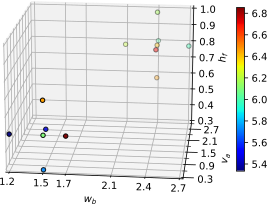
\includegraphics[width=\columnwidth]{sources/testing/straight_sample_points.pdf}
		\caption{Sampled points}
		\label{fig:test_points_straight}
	\end{subfigure}
	\caption{Experimental setup of straight design.}
\end{figure}


\todo{Further results are listen below.}




\subsubsection{Diagonal}
Because with a given $L=\SI{3.6}{\milli\meter}$, $h=\SI{0.2}{\milli\meter}$ and $\wa=\SI{0.6}{\milli\meter}$ the remaining design space is only one-dimensional,
we can simply sample various points along $\wb$: $(0.6, 1.2, 1.8, 2.4, 3.0, 3.6)$.
Again each specimen contains 5 cells in the horizontal direction, but 13 repetition in Z.
Extra finger beams are added to the sides of the specimen to prevent any part of the beam to be less than $2\wmin=\SI{0.6}{\milli\meter}$ wide.
See \cref{fig:test_diagonal_boundary_cells}.

\begin{figure}
	\centering
	\begin{subfigure}[B]{.24\columnwidth}
		\centering
		\includegraphics[width=\columnwidth]{sources/testing/diagonal_sample.jpg}
		\caption{Example print mesh}
		\label{fig:test_diagonal_boundary_cells}
	\end{subfigure}
	\begin{subfigure}[B]{.24\columnwidth}
		\centering
		\includegraphics[width=\columnwidth]{sources/testing/straight_print.jpg}
		\caption{Example print}
	\end{subfigure}
	\begin{subfigure}[B]{.5\columnwidth}
		\centering
		%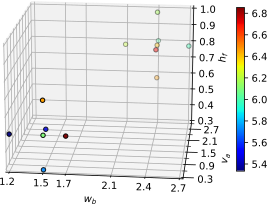
\includegraphics[width=\columnwidth]{sources/testing/straight_sample_points.pdf}
		\caption{Comparison of results to analytical model}
	\end{subfigure}
	\caption{Experimental setup of diagonal design.}
\end{figure}




\subsubsection{Dovetail interlocking}
suture; trapezoidal design for interlocking

jigsaw; similar to suture, but with semicircles attached. Lmax violated.

parameters, optimized using homogenous max tensile stress.


\subsection{Results}
figure for all printed models what the boundaries look like;
figure of gcode toolpaths;
max strength calculation

printing results; max strength table; some force-displacement figures

tables and figures comparing to model and FEM

\section{Discussion}


\subsection{Comparison of interlocking structures}

\subsection{Limitations}




\subsection{Applications}
Rigid + soft, rigid + chemically resistant.

Prosthetic hand, robotic gripper.


\section{Conclusion}

\subsection{Future work}
Big future

\section*{References}
\interlinepenalty=100000 % prevents pdfendlink ended up accross pages error. see https://tex.stackexchange.com/a/449633/129190
\bibliography{99_mybib}


%\begin{appendices}
%\input{19_edge_discretization}
%\end{appendices}

\end{document}
